\chapter{Algorithm to implement Palaniswamy's method}
In previous chapter has presented the method which we have used to estimate the landmarks on biological image based on the article of Palaniswamy. This chapter describe the implementation of the algorithms and additional operations that we have had to use to support for extraction of landmarks.
\section{Features extraction}
\subsection{Image preprocessing}
As discuss in previous, we use the thresholding technique to pre-process the image. As we know about thresholding technique, with a threshold value \textbf{``t"}, we can decrease the noise and obtain the interested features. The output of this technique is a binary image, which is generally used used to extract the features. The threshold value is defined by the histogram analysis (see figure \ref{fig:31}).
\begin{figure}[h!]
\centering
\subfloat[Image with noise]{\label{fig:seg_211}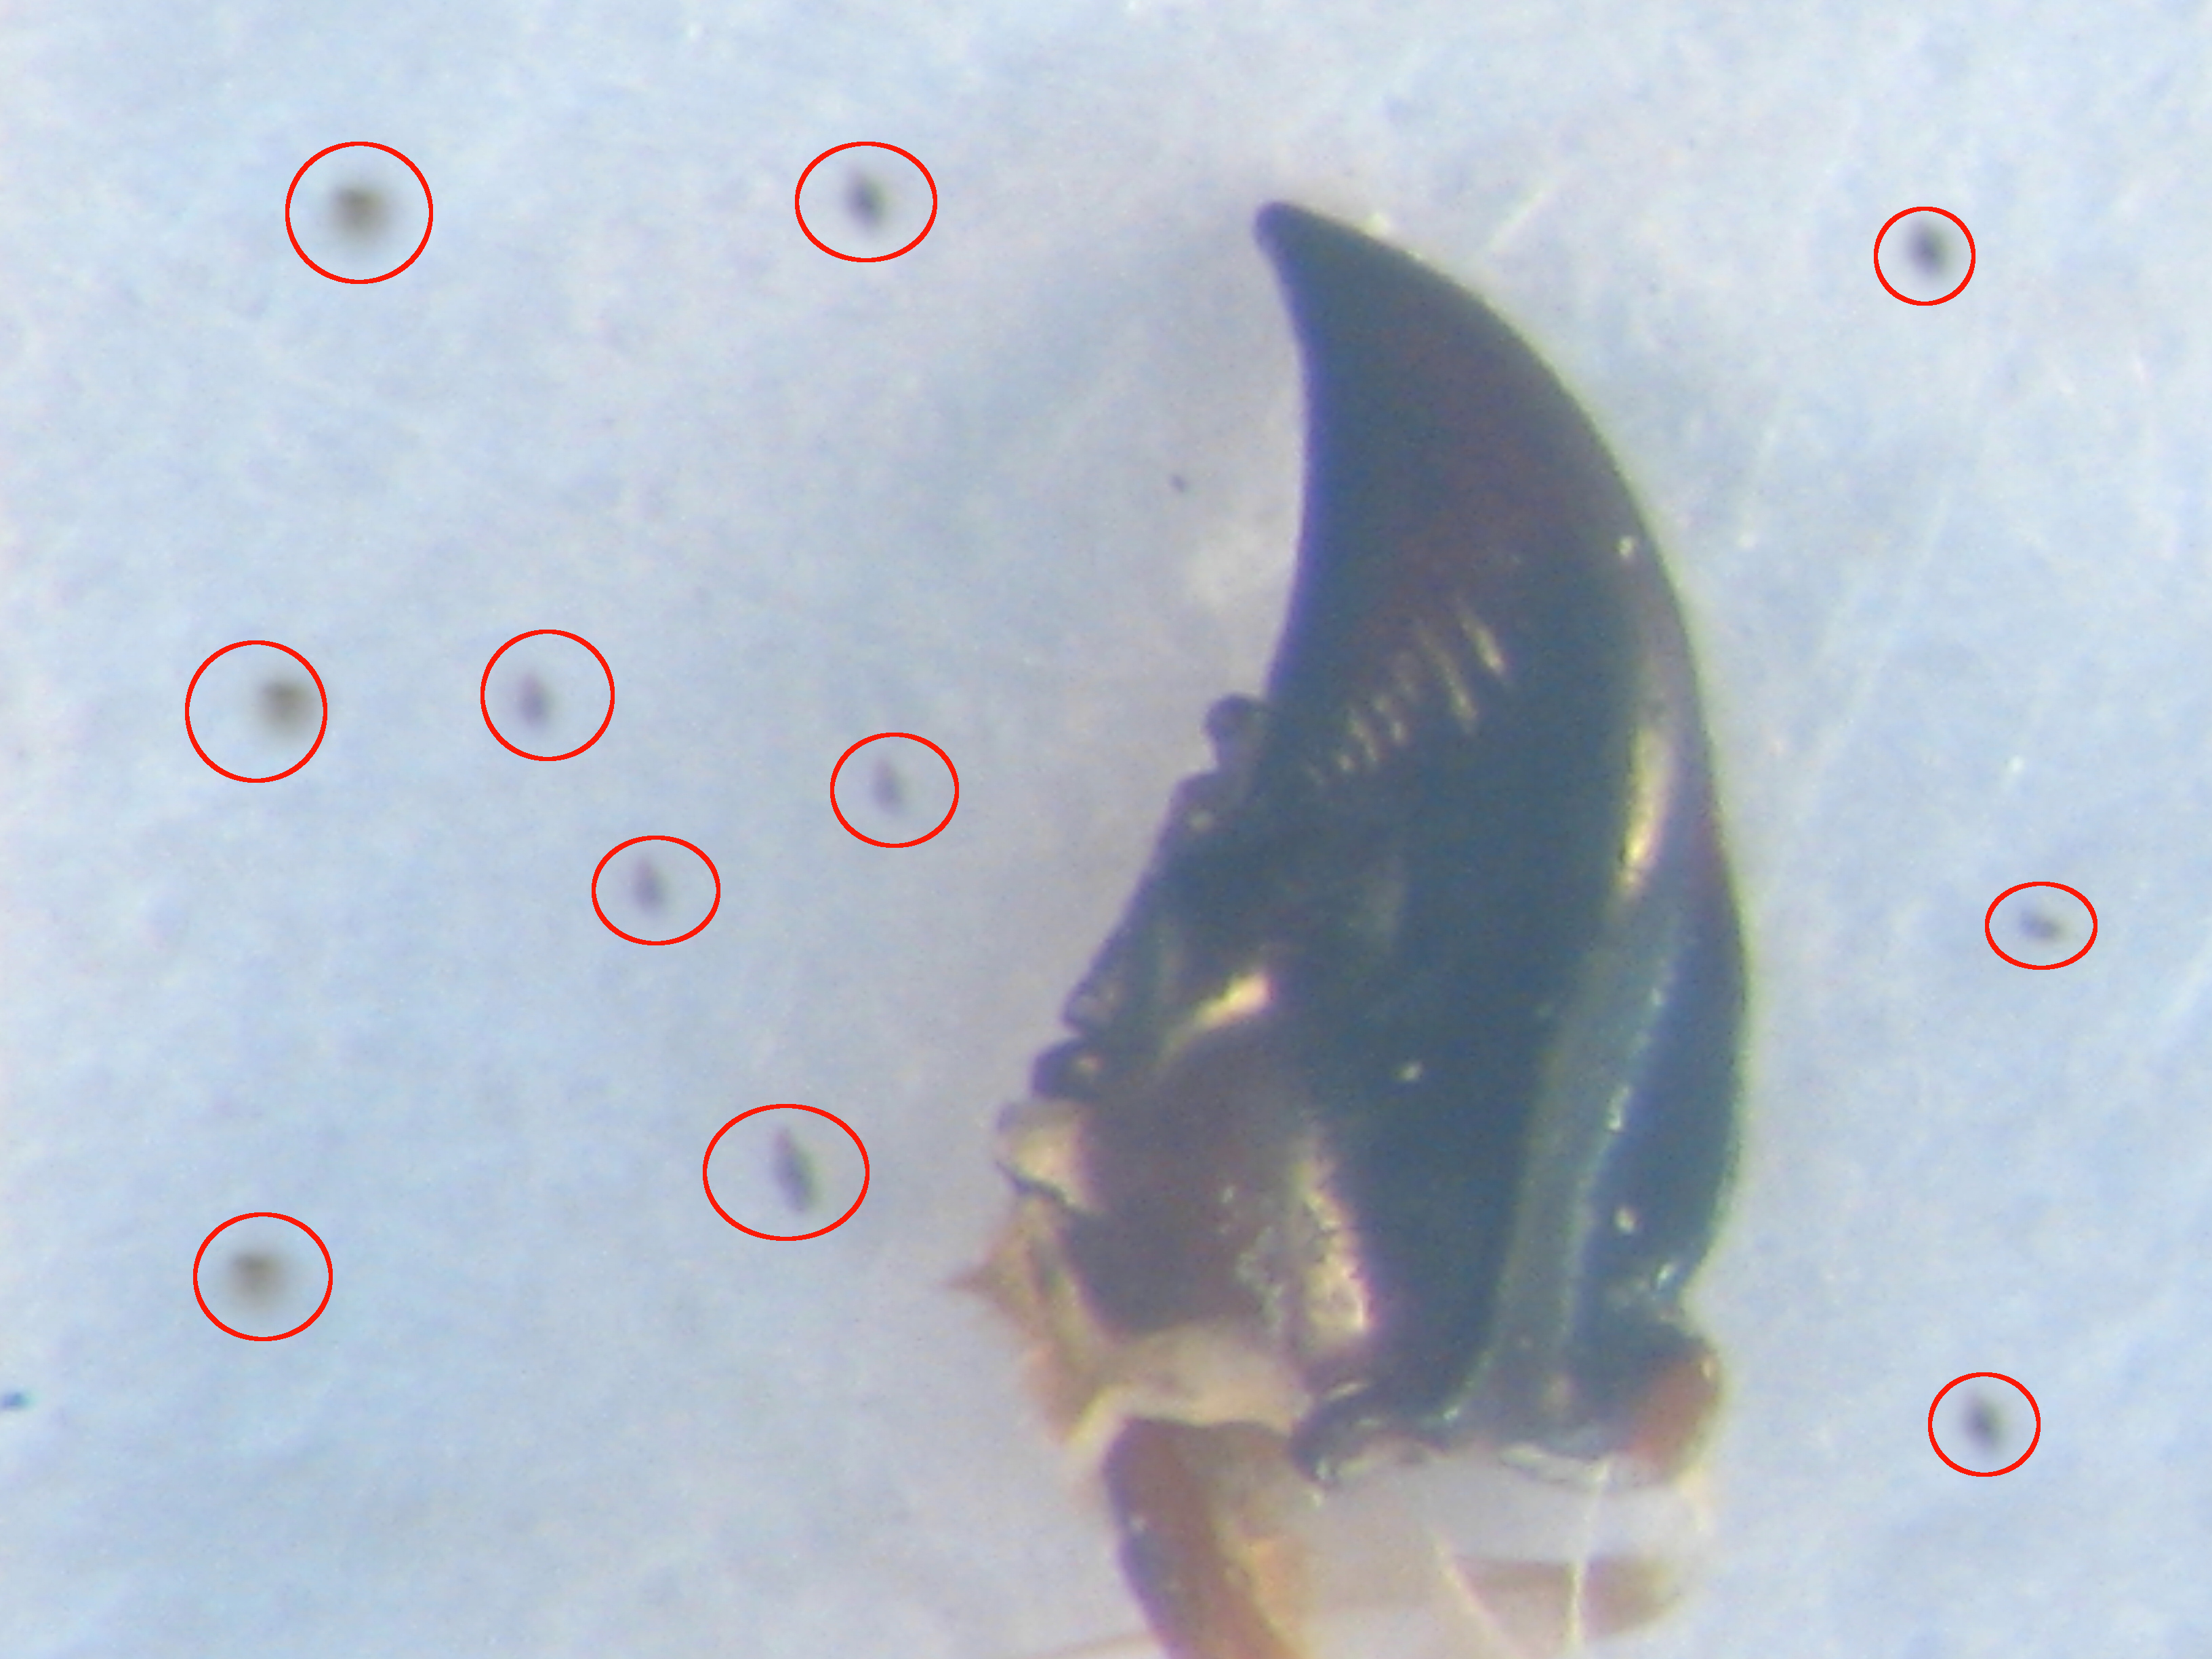
\includegraphics[width=0.4\textwidth]{./images/md019n}}~~
\subfloat[Image without noises]{\label{fig:seg_212}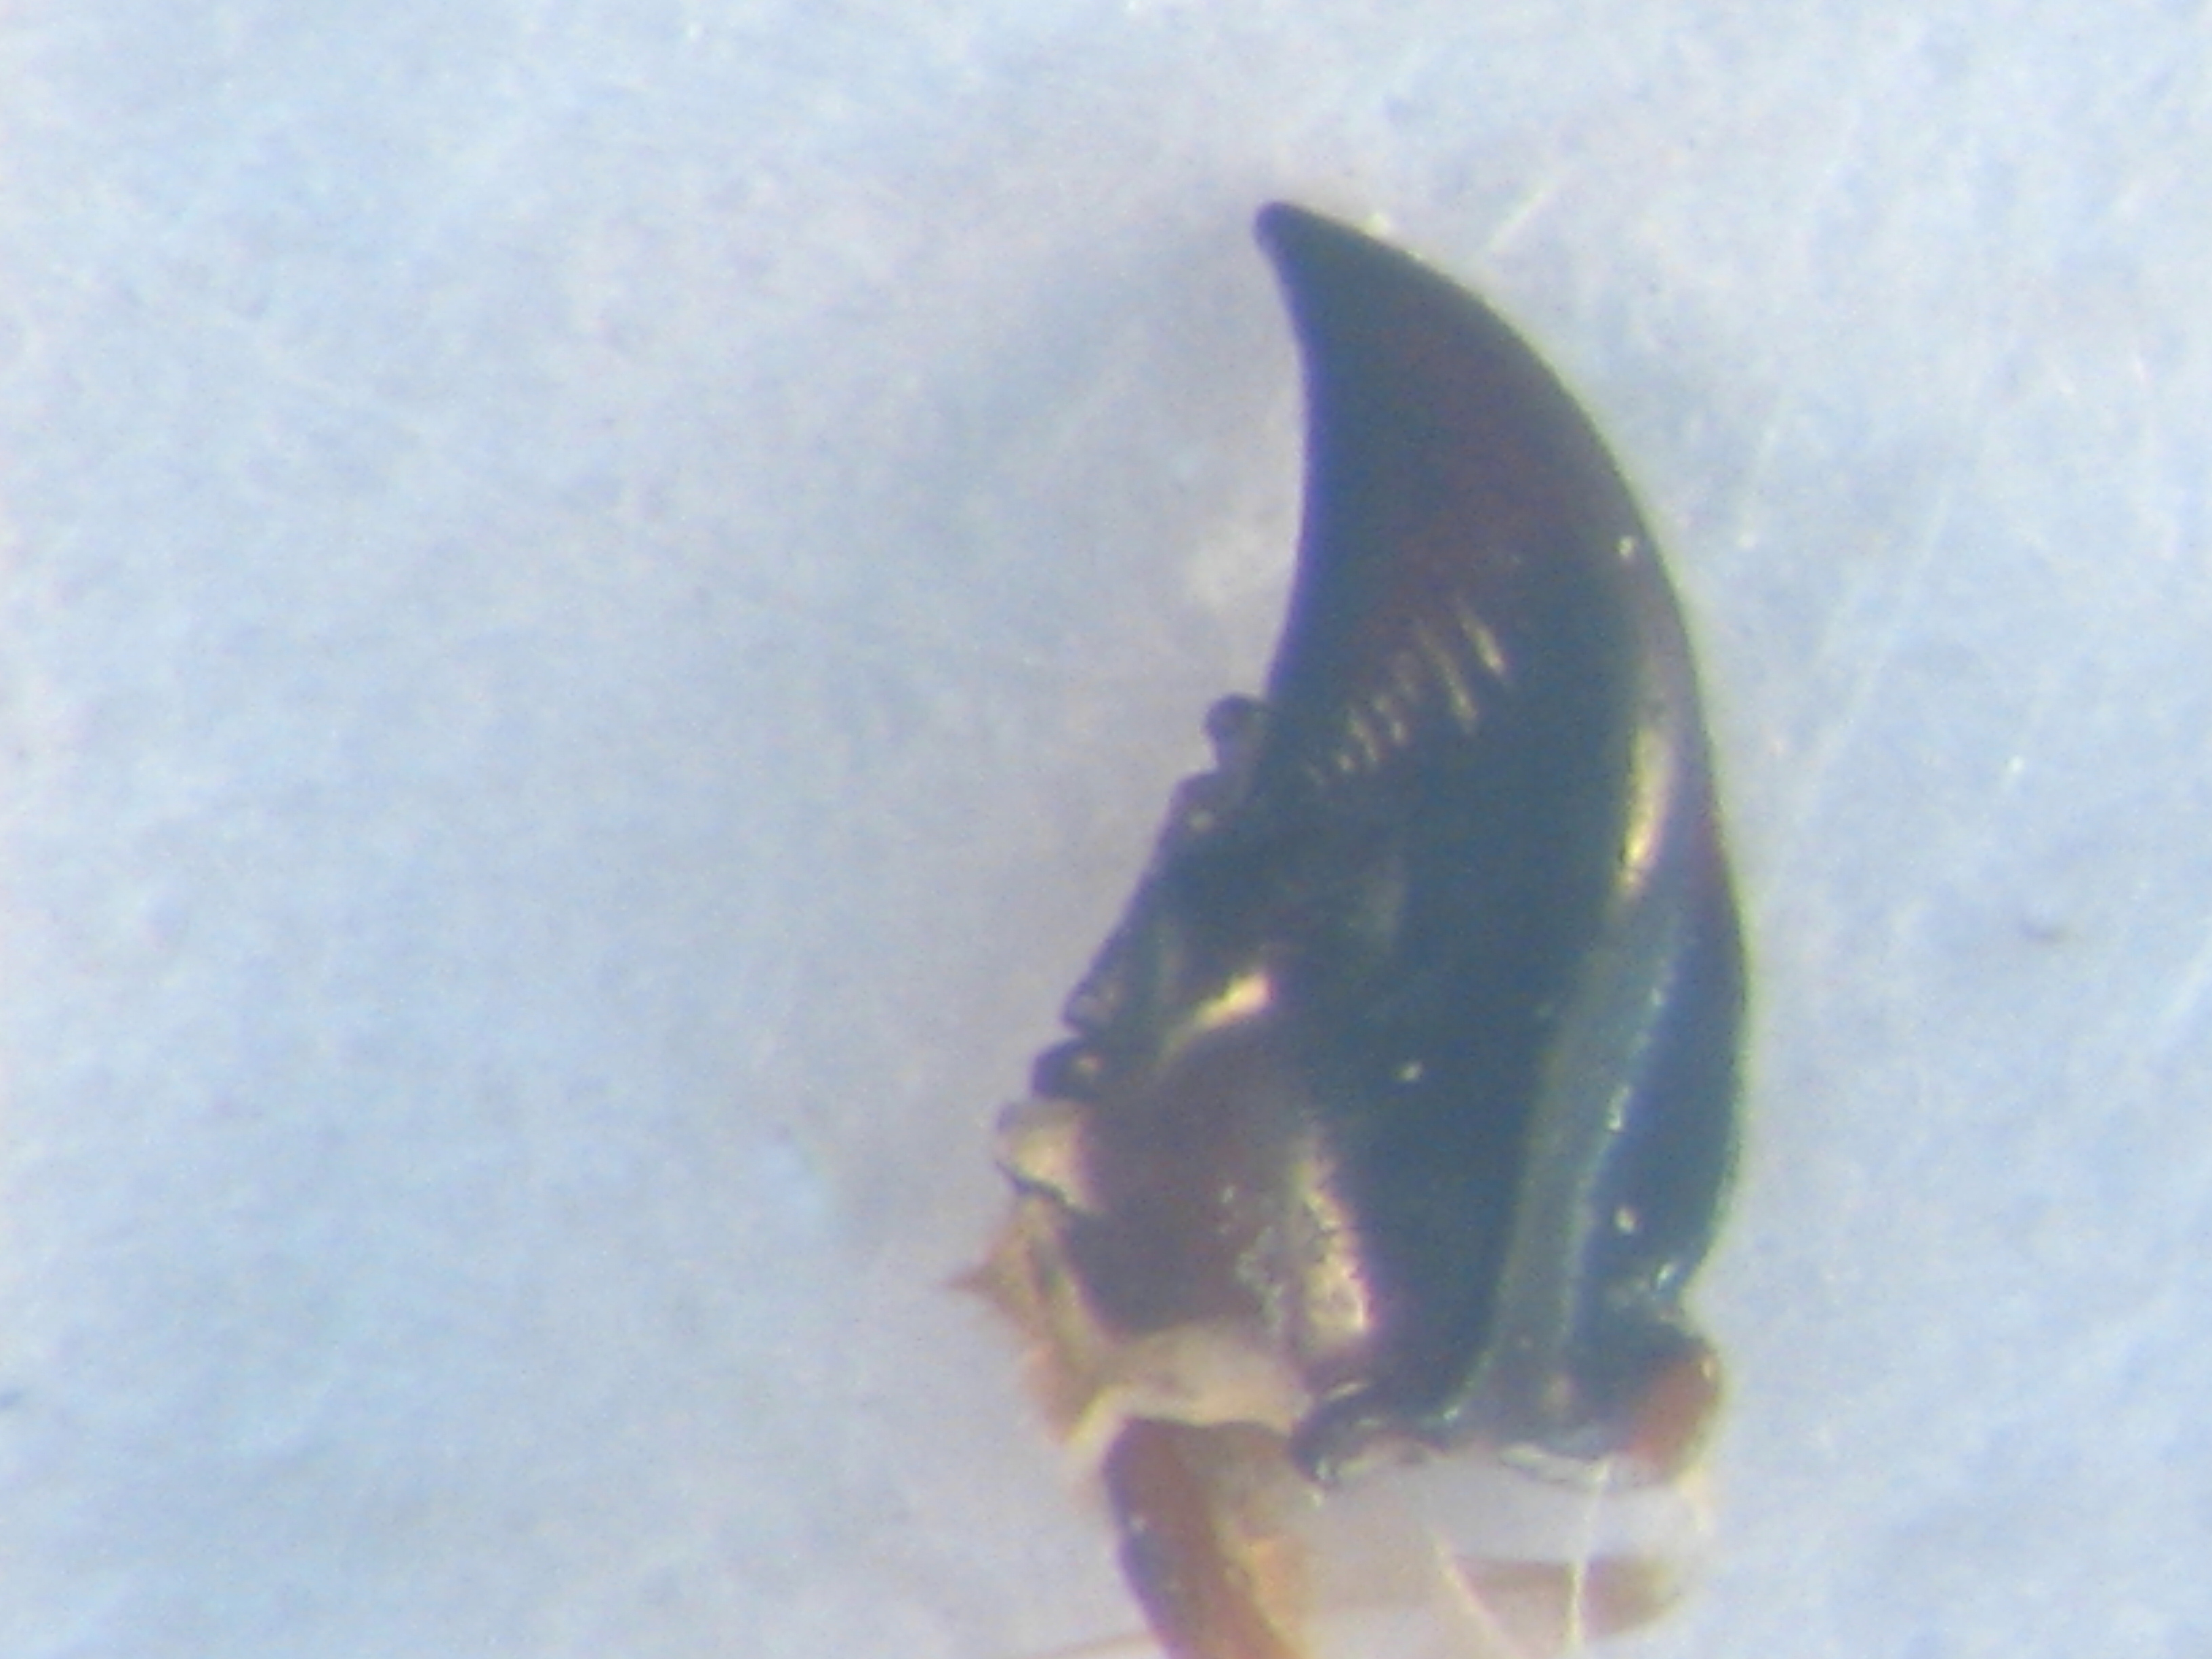
\includegraphics[width=0.4\textwidth]{./images/md019no}}
\caption{Example about noises in image}
\label{fig:31}
\end{figure}~\\
Based on the histogram of the original image, we compute the mean and the median of this histogram. With the histogram obtained, we split it into two parts: the first part starts from the beginning to the limit value (the limit value is the smallest value between mean and median); the second part, starts from the limit value to the end of the histogram. For each part, we find the maximum, minimum value and calculate the mean of them. The threshold value \textbf{``t"} obtained by the mean of the two mean values in two parts of histogram (as algorithm \ref{al_preprocess}).\\
\begin{figure}[h!]
\centering
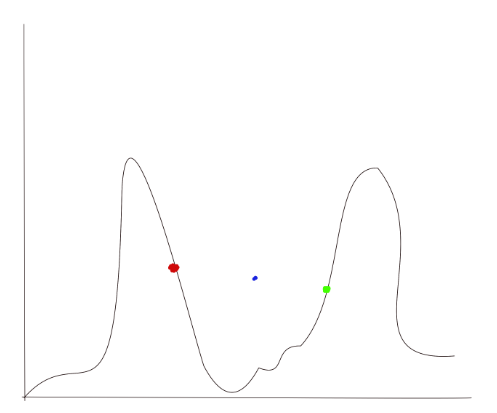
\includegraphics[width=0.6\textwidth]{./images/hist}
\caption{Analysis the histogram of image}
\label{fig:32}
\end{figure}~\\
Figure \ref{fig:32} present the histogram of an image. In this histogram, the threshold value (blue point) is indicated by mean of two means value of two parts (red and green point). This value is used in the method to pre-process image and to extract the edge from image.\\
\IncMargin{1em}
\begin{algorithm}[H]
\fontsize{10pt}{10pt}\selectfont
\setstretch{1}
\SetAlgoLined
\Indm 
\KwData{inputImage: the input image}
\KwResult{outputImage: the image after processing}
\Indp
Convert the input image into gray scale image\;
Calculate the histogram on gray scale image and store the result in $histogram$ variable \;
Compute the $mean$ value and $median$ value of histogram\;
$limit \leftarrow (mean > median$ ? $median : mean)$\;
$limitSub \leftarrow ((limit >= 120)$ ? $(limit - 25) : (limit - 5))$\;
Declare some variables: $int$ $imax \leftarrow -1, max \leftarrow -1$\;
\For{$i \leftarrow$ 0 to $limitSub$}{
	\If{$histogram[i]$ $>$ $max$}{
		$max$ = $histogram[i]$\;
		$imax$ = $i$\;
	}
}
Declare some variables: $int$ $imin \leftarrow -1, min \leftarrow max$\;
\For{$k \leftarrow$ imax to $limit$}{
	\If{$histogram[k]$ $<$ $min$}{
		$min$ = $histogram[k]$\;
		$imin$ = $k$\;
	}
}
Declare some variables: $int$ $max2 \leftarrow -1, imax2 \leftarrow -1$\;
\For{$j \leftarrow limit $ to $end\_of\_histogram$}{
	\If{$histogram[j]$ $>$ $max2$}{
		$max2$ = $histogram[j]$\;
		$imax2$ = $j$\;
	} 
}
$middle1 \leftarrow (imax1 + imin)/2$ \;
$middle2 \leftarrow (imax2 + imin)/2$ \;
$middle \leftarrow (middle1 + middle2)/2$ \;
Apply the threshold with threshold value is $middle$\;
\caption{Algorithm to get the threshold value and pre-process image}
\label{al_preprocess}
\end{algorithm}
\DecMargin{1em}
\subsection{Edges extraction}
The edges extraction are finished follows two steps:
\begin{itemize}
\item Edge extraction by applying Canny algorithm
\item Edge retrieve by applying function to get the contours.
\end{itemize} 
The threshold value used in Canny algorithm is the value used in the previous step (pre-process image), and the ratio between lower threshold and upper threshold is 1 : 3 (follows the article \cite{palaniswamy2010automatic} but have to be modified).

\iffalse
 This operation used from OpenCV library. The values provide for the parameters in Canny\footnote{http://docs.opencv.org/modules/imgproc/doc/feature\_detection.html\#canny} operator are:
 \fi 
 
An implementation of Canny algorithm is available in the OpenCV library\footnote{http://docs.opencv.org/modules/imgproc/doc/feature\_detection.html\#canny}, the different parameters required by the method are:
\begin{itemize}
\item Source image: the input image after pre-processing (in grayscale mode),
\item Destination image: the output image,
\item Lower threshold value: the lower threshold value (\textit{t}),
\item Upper threshold value: the upper threshold value (\textit{3t}),
\item Kernel size: size of kernel, aperture for the Sobel operator (5 pixels).
\end{itemize}
To retrieve the contours after applying the Canny algorithm, we apply the method to analysis the structure of topology to get the edges. This method also provided by OpenCV library(\textbf{findContours} function). It will return a list of the edges, and each edge was presented by a list of points. 
The parameters used in find contours method are as follows:
\begin{itemize}
\item Source: the binary input image (output of Canny algorithm),
\item Contours: the output. Each contours is stored in a vector of points,
\item Hierarchy: optional output vector, containing information about the image topology,
\item Mode: contours retrieve mode,
\item Method: contours approximation method,
\item Offset: optional offset by which every contour point is shifted.
\end{itemize}
\subsection{Edge fragmentation}
The steps of the method used to fragment the edges as follows:
\begin{itemize}
\item Establish a line \textit{``l"} between two endpoints of the edge.
\item For each point on edge, we compute the perpendicular distance from it to the line \textit{``l"} and keep the point which has the maximum perpendicular distance.
\item If the maximum perpendicular distance from a point on edge to the line \textit{``l"} is greater than $\alpha$, then the edge is splitted at this point. The value chosen for $\alpha$ in the program is 3 ($\alpha = 3$) because this value is enough minimum for stop fragmenting the edge.
\item Reprocess both parts which was obtained from step 3.
\item The algorithm continues until all edges fragments are represented.
\end{itemize}
And the algorithm is presented as follows (algorithm \ref{app_lines}):\\
\IncMargin{1em}
\begin{algorithm}[H]
\Indm 
\setstretch{0.9}
\SetAlgoLined
\KwData{listPoints: list of points which presented the edge}
\KwResult{Queue of ``step" points on the edge}
\Indp
Declare the first endpoint: $p0 \leftarrow listPoints[0]$\;
Declare the second endpoint: $pend \leftarrow listPoints[size - 1]$, \textit{size} is the size of \textit{listPoints}\;
Set up a straight line between the two endpoints $p0, pend$ (line $d$)\;
Initialization the max value: $maxDistance  \leftarrow 0 $\;
Declare a ``split point": $imax \leftarrow 0$ \; 
Declare a variable: $distance \leftarrow 0$\;

\For{ point $p$ in $listPoints$}{
	$distance \leftarrow$ from $p$ to line $d$\;
	\If{distance $>$ max\_distance}{
		$maxDistance$ $\leftarrow$ $distance$\;
		$imax$ $\leftarrow$ position of $p$\;
	}
}
\If{$maxDistance$ $>$ 3 }{
	split the list of points at $imax$ and put into 2 parts $(part1, part2)$\;
	Pre-process on $part1$\;	
	Pre-process on $part2$\;
}
\If {$p0$ does not exist in result queue}{
	push $p0$ into queue\;\tcp{queue is a variable of class}
}
\If {$pend$ does not exist in result queue}{
	push $pend$ into queue\;\tcp{queue is a variable of class}
}
\caption{Algorithm to segment an edge into approximate lines}
\label{app_lines}
\end{algorithm}\DecMargin{1em}
\section{Features description (Pairwise Geometric Histogram)}
The PGH is represented as two-dimension matrix. An axis presents for angle information (rows) and another presents for perpendicular distance information (columns). Based on the accuracy of requirements, the range of angle and distance axis can be changed. In default, the range of angle axis and distance axis are ($0$ - $\pi$) and 500, respectively.
\subsection{PGH constructor}
The proceed to construct the PGH was described in below:
\begin{itemize}
\item Choose the \textbf{reference line} (other lines called \textbf{object lines}),
\item For each object line, compute the angle between it and reference line (assigned \textbf{angle}); and the perpendicular distance from two endpoints of object line to reference line (assigned \textbf{dmin} and \textbf{dmax}),
\item Recording the perpendicular distance and the angle relation between reference line and the object lines into the matrix (PGH histogram). The recording was finished by marking the cells at row \textbf{angle} and from column \textbf{dmin} to column \textbf{dmax}.
\end{itemize}
The construction of local PGH and global PGH is the same, the only difference is the global PGH includes many local PGH and they are presented on the same matrix.
\iffalse
\subsection{Global PGH constructor}
The duration to construct the global PGH also similar to local PGH. Especially, the information of all local PGH are presented in the same matrix.
\fi
\subsection{PGH matching}
Follows the analysis, the Bhattacharya metric used to compute the similarity between two models. The models were presented by the global PGH which should be have the same size (width and height). The algorithm to compute the Bhattacharya metric between two models is described as below (algorithm \ref{al_bhattacharya}):\\
\IncMargin{1em}
\begin{algorithm}[H]
\Indm 
\setstretch{1}
\SetAlgoLined
\KwData{
	\begin{itemize}
		\item model: the global PGH of model
		\item scene: the global PGH of scene
	\end{itemize}
}
\KwResult{Measure distance between model and scene}
\Indp
$width$ $\leftarrow$ the width of model (or scene) PGH\;
$height$ $\leftarrow$ the height of model (or scene) PGH \;
$modelEntries$ $\leftarrow$ the total entries of model PGH\;
$sceneEntries$ $\leftarrow$ the total entries of scene PGH\;
$double$ $distance, distance1, distance2$\;
\For{ $size\_t$ $i$ from $0$ to $width$}{
	\For{$size\_t$ $j$ from $0$ to $height$}{
		$distance1$ = $sqrt($ $model[i][j] / modelEntries$ $)$\;
		$distance2$ = $sqrt($ $scene[i][j] / sceneEntries$ $)$\;
		$distance$ += $distance1$ * $distance2$\;
	}
}
\caption{Algorithm to compute the measure metric between 2 PGH using Bhattacharya}
\label{al_bhattacharya}
\end{algorithm}
\DecMargin{1em}~\\
Besides the Bhattacharya metric, we may choose another metric to find the similarity the histograms, such as: \textbf{Chi-squared} metric and \textbf{Intersection} metric. The forms are presented as below:\\[0.5cm]
\textbf{Chi-squared metric:}
\begin{center}
\begin{equation}\label{eq:2}
d_{Chi-squared} (H_{i}H_{j}) = \frac{\sum\limits_{\theta}^{\pi}\sum\limits_{d}^{d_{max}}(\frac{(H_{i}(\theta,d) - H_{j}(\theta,d))^{2}}{(H_{i}(\theta,d) + H_{j}(\theta,d))})}{2}
\end{equation}
\end{center}
\textbf{Intersection metric}
\begin{center}
\begin{equation}\label{eq:3}
d_{Intersection} (H_{i}H_{j}) = \sum\limits_{\theta}^{\pi}\sum\limits_{d}^{d_{max}}min(H_{i}(\theta,d), H_{j}(\theta,d))
\end{equation}
\end{center}
The significance of parameters in formula (\ref{eq:2}) and (\ref{eq:3}) are similar to formula (\ref{eq:1}). For the Bhattacharyya and Intersection metric, the perfect match is 1 and the total mismatch is 0. The result is opposite to Chi-squared metric (0 for perfect match and 1 for total mismatch).\\[0.2cm]
These are two other ways to define metric but as no better result has been obtained. We choose to keep the Bhattacharya metric to match histograms.
\section{Global pose estimation (Probabilistic Hough Transform)}
The core of PHT uses vote procedure to find the model's position in the scene image. The process to estimate the model's landmarks on scene image includes the steps as follows:
\begin{itemize}
\item Choose an arbitrary point in the model as a reference point,
\item For each pair lines in the model, calculating and recording the perpendicular distance and angle from the reference point to each line. And save the information into a table,
\item Create an two-dimensional accumulator, one dimension for the angle and the other for the perpendicular distance,
\item For each pair lines in the scene, finding the entry correspond to the position, orientation and scale. Increasing the value at correlative cell in the accumulator (indicate by the angle and distance),
\item Compute the maximum value in the accumulator,
\item Indicating the pair of scene lines and the entry with maximal value of accumulator,
\item Extending the perpendicular lines of the pair belong to scene lines at the appropriate position. The intersection of them is the location of the model's reference point in the scene image.
\end{itemize}
\subsection{Training process}
The training process starts with creating the model's \textbf{reference table}. Each entry in reference table includes pair of model lines and geometric information (angle and perpendicular distance) from each line to reference point. To reduce the time complexity processing during training process, we consider the ``closest pair lines". The algorithm considers a pair of closest lines and constructs the reference table as follows (algorithm \ref{al_closestlines} and \ref{al_refTable}):\\[0.2cm]
\begin{algorithm}[H]
\Indm 
\setstretch{1}
\SetAlgoLined
\KwData{line1 (the first line), line2 (the second line)}
\KwResult{Two line closet or not (bool)}
\Indp
$distance1$ $\leftarrow$ distance from the first endpoint of $line1$ to $line2$\;
$distance2$ $\leftarrow$  distance from the second endpoint of $line1$ to $line2$\;
\If {$line1.length() > $ 60 and $line2.length() > $60  \\
		and $line1$ not parallel with $line2$\\
		and ($distance1$ $<=$ 5 or $ditance2$ $<=$ 5 )}{
	$return$ $true$\;
}
return $false$\;
\caption{Algorithm to consider the closest lines}
\label{al_closestlines}
\end{algorithm}~\\[0.2cm]
\begin{algorithm}[H]
\Indm 
\setstretch{1}
\SetAlgoLined
\KwData{lines (a list of lines), refPoint (the reference point)}
\KwResult{The reference table}
\Indp
Declare the reference table $refTable$ \;
\For{ line $i$ in $lines.size()$}{
	\For{line $j$ in $lines.size()$}{
		\If{i $!=$ j and $line(i)$ closet with $line(j)$}{
			Compute the angle and perpendicular distance from $line(i)$ to $refPoint$\;
			Compute the angle and perpendicular distance from $line(j)$ to $refPoint$\;
			Create an entry to store pair of lines and its information \;
			Add the entry into reference table \;
		}
	}
}
return $refTable$ \;
\caption{Algorithm to construct the reference table}
\label{al_refTable}
\end{algorithm}~\\
The training process is finished by finding a pair of scene lines agree with a pair of model lines. An accumulator was created to store each agreement between the pair of scene lines and the pair of model lines. For each pair of scene lines, we find its exist in the reference table and increase the value at correspondence position in accumulator. At the end, we obtain a pair of scene lines and pair of model lines correspondence with the maximum value in accumulator. The below algorithms describe the steps to finish the training process (algorithm \ref{al_agreelines},  \ref{al_similarlines}):\\[0.2cm]
\begin{algorithm}[H]
\Indm 
\setstretch{1}
\SetAlgoLined
\KwData{line1 (the first reference line), line2 (the second reference line), sline1 (the first scene line), sline2 (the second scene line)}
\KwResult{Two pair lines similar or not (bool value)}
\Indp
$angle1$ $\leftarrow$ angle between $line1$ and $line2$\;
$angle2$ $\leftarrow$ angle between $sline1$ and $sline2$\;
$mdistance$ $\leftarrow$ sum of perpendicular distance from two endpoints of $line1$ to $line2$\;
$sdistance$ $\leftarrow$ sum of perpendicular distance from two endpoints of $sline1$ to $sline2$\;
\If{$abs(ange1$ - $angle2) < 1$ \\
	$and$ $abs(line1.length()/sline1.length()$ - $line2.length()/sline2.length()) < 1$ \\
	$and$ $abs(mdistance$ - $sdistance) < 2$}{
	return $true$\;
}
return $false$ \;
\caption{Algorithm to check the agreement between two pair lines}
\label{al_agreelines}
\end{algorithm}~\\[0.2cm]
\iffalse
\begin{algorithm}[H]
\Indm 
\setstretch{1}
\SetAlgoLined
\KwData{refTable (the reference table), slines (pair of scene lines)}
\KwResult{The entries in reference table similar with pair of scene lines}
\Indp
Declare the return entries in reference table $entries$ \;
\For{ entry $et$ in $refTable$}{
	\If{agree between lines in entry and $slines$}{
		put the entry $et$ into list of entries $entries$\;
	}
}
return $entries$ \;
\caption{Algorithm to find the agreement of pair scene lines in model}
\label{al_findalines}
\end{algorithm}~\\[0.2cm]
\fi
\begin{algorithm}[H]
\Indm 
\setstretch{1}
\SetAlgoLined
\KwData{lines (a list of scene lines), refTable (reference table)}
\KwResult{The pair of scene lines which has the best vote and the corresponding entry in reference table}
\Indp
Create an accumulator, $acc$\;
Declare the reference table $refTable$ \;
\For{ line $i$ in $lines.size()$}{
	\For{line $j$ in $lines.size()$}{
		\If{i $!=$ j and $line(i)$ closet with $line(j)$}{
			Find the agreement of pair scene lines in mode\;
			Increase the value in $acc$ with correspondence position\;
			Marked the maximum value, pair of scene lines and entry in reference table\;
		}
	}
}
Indicate the pair of scene lines has the best vote\;
Indicate the pair of model lines correspondence with pair of scene lines\;
\caption{Algorithm to find similar pairs between model image and scene image}
\label{al_similarlines}
\end{algorithm}
\subsection{Estimation process}
At the end of training process, we obtained similar pairs between model image and scene image. In this step, the model reference point estimated by extending the perpendicular lines of the pair of scene lines at the appropriate position. The algorithm to find the model reference point in scene image as follows (algorithm \ref{al_refPointScene}): \\[0.2cm]
\begin{algorithm}[H]
\Indm 
\setstretch{1}
\SetAlgoLined
\KwData{pair of scene lines, pair of model lines (entry in reference table)}
\KwResult{The position of model reference point in scene image}
\Indp
Find the match lines between pair of scene lines and pair of model lines\;
Find two lines which parallel with pair of scene lines that the distance between them following the distance in entry\;
Find the intersection between two parallel lines\;
\caption{Algorithm to find position of model reference point in scene image}
\label{al_refPointScene}
\end{algorithm}~\\[0.2cm]
By finding the reference point, the landmarks in the scene image can be estimated by calculating the relatedness between the reference point and the reference landmarks. Besides, we also record the difference about rotation, orientation and scale between the model image and the scene image.
\section{Landmarks refinement}
Refining landmarks is finished by applying the cross-correlation. In this case, the template is a region around each landmark in model image and the image is also a region around the Hough landmark detection (the landmarks estimated in previous stage) in scene image. Hence, to save the processing time, before applying the cross-correlation, the scene image is rotated to match with model. The angle difference between the model image and the scene image is obtained from Hough estimation in the previous stage.\\[0.2cm]
For each landmark in the model image, we create a bounding box around the landmarks with an arbitrary size and use landmark as a center point. When create the bounding box, we need to keep the distance between left corner to the landmarks, because sometimes, with the landmark position, the size of bounding box can be over the size of image. Use this box as a \textit{template}. Doing the same with each estimated landmarks on scene image but using a larger size to create the \textit{small image}. Then applying the cross-correlation between \textit{template} and \textit{small image}. The results obtained store the location where the template matches the image. From these position, we indicate the position of each landmark of reference image on scene image. The algorithm to create the bounding box around a landmark is described follows (algorithm \ref{al_boundingbox}):\\[0.2cm]
\begin{algorithm}[H]
\Indm 
\setstretch{1}
\SetAlgoLined
\KwData{image (reference image), landmark (location of a reference landmark), tsize (size of bounding box), distance (to keep the distance from the landmark to bounding box)}
\KwResult{A matrix represented for bounding box of landmark}
\Indp
Get the matrix of image (image presented by matrix): $Mat matImg = image.getMatrix()$\;
\tcp{Indicate the top left-corner of bounding box:}
$int$ $lx = (landmark.x - tsize/2) < 0$ ? $0$ : $(landmark.x - tsize/2)$\;
$int$ $yx = (landmark.y - tsize/2) < 0$ ? $0$ : $(landmark.y - tsize/2)$\;
\tcp{Keep the distance from the landmark to bounding box}
$distance.x = landmark.x - lx$\;
$distance.y = landmark.y - ly$\;
\tcp{Indicate the low right-corner of bounding box}
$int$ $lx2 = (landmark.x + tsize/2) > matImg.cols$ ? $matImg.cols$ : $(landmark.x + tsize/2)$\;
$int$ $yx2 = (landmark.y + tsize/2) < matImg.rows$ ? $matImg.rows$ : $(landmark.y + tsize/2)$\;
\tcp{Create the bounding box around landmark}
$Mat$ $box(matImg,Rect(lx,ly,lx2 - lx, ly2 - ly))$\;
return the $box$;
\caption{Algorithm to create a bounding box around a landmark}
\label{al_boundingbox}
\end{algorithm}~\\[0.2cm]
The below algorithm (algorithm \ref{al_ccross}) describe a method to refine the estimated landmarks on a scene image by using cross-correlation. Remember that, before applying the cross-correlation, the scene image is rotated to match with the model; and the angle used to rotate is the sum of the angle difference between the scene line and model line to which it matched and the angle difference between the two pairs of the similar lines.\\
Cross correlation method allows us compare the template overlapping the image. When the template slide over each pixel on image, the coefficient between them is calculated and stored in a array.\\[0.2cm]
After finished correlation, we get the value and the position of the maximum value.\\[0.2cm]
\begin{algorithm}[H]
\Indm 
\setstretch{1}
\SetAlgoLined
\KwData{refImage (reference image), sceneImage (the scene image), lmpath (file path store the reference landmarks)}
\KwResult{A list of landmarks on scene image}
\Indp
Get the reference landmarks from file and store in list $refLandmarks$\;
Create a variable to store the new landmarks: $sceneLandmarks$\;
Estimate the reference landmarks ($refLandmarks$) in scene image using probabilistic Hough transform and save into a variable: $esLandmarks$\;
\tcp{Get the matrix of scene image}
$sceneMatrix$ = $sceneImage.getMatrix()$\;
Rotate the scene matrix with appropriate angle\;
\For{ variable $i$ in $esLandmarks.size()$}{
	\tcp{Get the reference landmark}
	$Point$ $refPoint$ = $refLandmarks.at(i)$\;
	\tcp{Create a bounding box of reference landmark $refPoint$} 
	$Mat$ $template$ = $createTemplate(refImage, refPoint, size )$\;
	\tcp{Get the estimate landmark}
	$Point$ $esPoint$ = $esLandmarks.at(i)$\;
	\tcp{Create a bounding box of estimate landmark $esPoint$} 
	$Mat$ $sceneImg$ = $createTemplate(sceneImage, esPoint, size )$\;
	Create the matrix to store the value when do the cross-correlation: $result$ \;
	\tcp{Apply the matching and store the result into matrix $result$}
	$cv::matchTemplate(sceneMatrix,template,result,CV\_TM\_CCORR\_NORMED$\;	
	\tcp{Get the maximum value and position in $result$ matrix}
	$double$ $maxValue, minValue$\;
	$Point$ $maxLoc, minLoc$\;
	$cv::minMaxLoc(result, \&minValue, \&maxValue, \&minLoc, \&maxLoc, Mat())$\;
	Compute the position of landmark from maximum position\;
	Push the landmark into the list $sceneLandmarks$\;
}
Return the list of landmarks\;
\caption{Algorithm to get the position of reference landmarks in scene image}
\label{al_ccross}
\end{algorithm}~\\
\section{Summary}
This chapter has presented the algorithms to implement the Palaniswamy's method. Besides the new operations, we have used the method from OpenCV library. The value of parameters are indicated by experiment. In the next chapter, we describe about the software and our examination based on the two datasets.